% Foliensatz: "AFu-Kurs nach DJ4UF" von DK0TU, Amateurfunkgruppe der TU Berlin
% Lizenz: CC BY-NC-SA 3.0 de (http://creativecommons.org/licenses/by-nc-sa/3.0/de/)
% Autoren: Sebastian Lange <dl7bst@dk0tu.de>
% Korrekturen: Lars Weiler <dc4lw@darc.de>

\documentclass[aspectratio=169]{beamer}

\usepackage[ngerman]{babel} % deutsche Worttrennung etc.
\usepackage[utf8]{inputenc} % UTF8 Text

\usepackage[super, comma, numbers, square, sort]{natbib}

\usepackage{hyperref}       % Hyperref Package für bessere Referenzen (todo)
\hypersetup{
	colorlinks=false,       %   false: boxed links; true: colored links
    %linkcolor=white,       %   color of internal links (change box color with linkbordercolor)
    citecolor=red,          %   color of links to bibliography
    filecolor=white,        %   color of file links
    urlcolor=blue           %   color of external links
}

\usepackage{multirow}
\usepackage{wasysym}  % Math Symbols like \permil
%\usepackage{colortbl}
%\usepackage{subscript}
%\usepackage{caption}
%\usepackage{setspace}
%\usepackage{xcolor}        % benutze CodeListe

% Footnote
%\usepackage{hanging}
%
%\setbeamertemplate{footnote}{%
%  \hangpara{2em}{1}%
%  \makebox[2em][l]{\insertfootnotemark}\footnotesize\insertfootnotetext\par%
%}


%\usepackage{pgf}
%\usepackage{tikz}
%\usetikzlibrary{arrows,automata}
%\usetikzlibrary{positioning}
%
%\tikzset{
%    state/.style={
%           rectangle,
%           rounded corners,
%           draw=black, very thick,
%           minimum height=2em,
%           minimum width=2pt,
%           inner sep=2pt,
%           text centered,
%           },
%}

%\usepackage{listings}
%\lstset{basicstyle=\small, numberstyle=\tiny, extendedchars=true, numbers=left, numbersep=5pt}
%\lstset{showtabs=false, showspaces=false, showstringspaces=false}
%%\lstset{backgroundcolor=\color{white!75!lightgray}, , frame=single}
%%\lstset{backgroundcolor=\color{white}}
%%\lstset{backgroundcolor=none}
%\lstset{keywordstyle=\color{blue!50!gray},  identifierstyle=\color{black}}
%\lstset{commentstyle=\color{green!50!gray}, stringstyle=\color{red!50!gray}}
%\lstset{language=C, fontadjust=true, tabsize=2, breaklines=true}
%\lstset{backgroundcolor=\color{white!75!lightgray}, caption=\lstname, frame=single}
%\lstset{emphstyle=\color{black}\fbox}
%
%% Keine "Listing:"-Caption
%\captionsetup{labelformat=empty,labelsep=none}
%
%% für mathematische Umgebungen
%\usepackage{amsmath,amsfonts,amssymb}
%
%\lstdefinestyle{Bash}{
%language=Bash,
%frame=single,
%rulecolor=\color{black},
%backgroundcolor=\color{gray!50},
%keywordstyle=\color{black},
%identifierstyle=,
%commentstyle=\color{black},
%stringstyle=\color{magenta!65!white},
%showstringspaces=false,
%basicstyle=\footnotesize\ttfamily\color{black},
%numbers=none,
%breaklines=true,
%captionpos=b
%}

%\usepackage{listings}
%
%\lstdefinestyle{basic}{
%    captionpos=t,%
%    basicstyle=\footnotesize\ttfamily,%
%    numberstyle=\tiny,%
%    numbers=left,%
%    stepnumber=1,%
%    frame=single,%
%    showspaces=false,%
%    showstringspaces=false,%
%    showtabs=false,%
%    %
%    keywordstyle=\color{blue},%
%    identifierstyle=,%
%    commentstyle=\color{gray},%
%    stringstyle=\color{magenta}%
%}



% fließende Boxen haben keinen Abstand
%\fboxsep0mm

% inkludiere Creative Commons Helper
%%%%%%%%%%%%%%%%%%%%%%%%%%%%%%%%%%%%%%%%%%%%%%%%%%%%%%%%%%%%%%%%
%% ccBeamer 0.1, 2007-07-02                                   %%
%% Written by Sebastian Pipping <webmaster@hartwork.org>      %%
%% ---------------------------------------------------------- %%
%% Licensed under Creative Commons Attribution-ShareAlike 3.0 %%
%% http://creativecommons.org/licenses/by-sa/3.0/             %%
%%%%%%%%%%%%%%%%%%%%%%%%%%%%%%%%%%%%%%%%%%%%%%%%%%%%%%%%%%%%%%%%


%% Images
\newcommand{\CcImageBy}[1]{%
	
\includegraphics[scale=#1]{texdata/creative_commons/cc_by_30.pdf}%
}
\newcommand{\CcImageCc}[1]{%
	
\includegraphics[scale=#1]{texdata/creative_commons/cc_cc_30.pdf}%
}
\newcommand{\CcImageDevNations}[1]{%
	
\includegraphics[scale=#1]{texdata/creative_commons/cc_dev_nations_30.pdf}%
}
\newcommand{\CcImageNc}[1]{%
	
\includegraphics[scale=#1]{texdata/creative_commons/cc_nc_30.pdf}%
}
\newcommand{\CcImageNd}[1]{%
	
\includegraphics[scale=#1]{texdata/creative_commons/cc_nd_30.pdf}%
}
\newcommand{\CcImagePd}[1]{%
	
\includegraphics[scale=#1]{texdata/creative_commons/cc_pd_30.pdf}%
}
\newcommand{\CcImageSa}[1]{%
	
\includegraphics[scale=#1]{texdata/creative_commons/cc_sa_30.pdf}%
}
\newcommand{\CcImageSampling}[1]{%
	
\includegraphics[scale=#1]{texdata/creative_commons/cc_sampling_30.pdf}%
}
\newcommand{\CcImageSamplingPlus}[1]{%
	
\includegraphics[scale=#1]{texdata/creative_commons/cc_sampling_plus_30.pdf}%
}


%% Groups
\newcommand{\CcGroupBy}[2]{% zoom, gap
	\CcImageCc{#1}\hspace*{#2}\CcImageBy{#1}%
}
\newcommand{\CcGroupByNc}[2]{% zoom, gap
	\CcImageCc{#1}\hspace*{#2}\CcImageBy{#1}\hspace*{#2}\CcImageNc{#1}%
}
\newcommand{\CcGroupByNcNd}[2]{% zoom, gap
	\CcImageCc{#1}\hspace*{#2}\CcImageBy{#1}\hspace*{#2}\CcImageNc{#1}\hspace*{#2}\CcImageNd{#1}%
}
\newcommand{\CcGroupByNcSa}[2]{% zoom, gap
	\CcImageCc{#1}\hspace*{#2}\CcImageBy{#1}\hspace*{#2}\CcImageNc{#1}\hspace*{#2}\CcImageSa{#1}%
}
\newcommand{\CcGroupByNd}[2]{% zoom, gap
	\CcImageCc{#1}\hspace*{#2}\CcImageBy{#1}\hspace*{#2}\CcImageNd{#1}%
}
\newcommand{\CcGroupBySa}[2]{% zoom, gap
	\CcImageCc{#1}\hspace*{#2}\CcImageBy{#1}\hspace*{#2}\CcImageSa{#1}%
}
\newcommand{\CcGroupDevNations}[2]{% zoom, gap
	\CcImageCc{#1}\hspace*{#2}\CcImageDevNations{#1}%
}
\newcommand{\CcGroupNcSampling}[2]{% zoom, gap
	\CcImageCc{#1}\hspace*{#2}\CcImageNc{#1}\hspace*{#2}\CcImageSampling{#1}%
}
\newcommand{\CcGroupPd}[1]{% zoom
	\CcImagePd{#1}%
}
\newcommand{\CcGroupSampling}[1]{% zoom
	\CcImageSampling{#1}%
}
\newcommand{\CcGroupSamplingPlus}[1]{% zoom
	\CcImageSamplingPlus{#1}%
}


%% Text
\newcommand{\CcLongnameBy}{Attribution}
\newcommand{\CcLongnameByNc}{Attribution-NonCommercial}
\newcommand{\CcLongnameByNcNd}{Attribution-NoDerivs}
\newcommand{\CcLongnameByNcSa}{Attribution-NonCommercial-ShareAlike}
\newcommand{\CcLongnameByNd}{Attribution-NoDerivs}
\newcommand{\CcLongnameBySa}{Attribution-ShareAlike}

\newcommand{\CcNote}[1]{% longname
	This work is licensed under the \textit{Creative Commons #1 3.0 License}.%
}


% generelles Thema auswählen
\usetheme{Goettingen} %Berlin spart ohne Sidebar allerdings angenehm Platz
% AnnArbor | Antibes | Bergen | Berkeley | Berlin | Boadilla | boxes | CambridgeUS | Copenhagen | Darmstadt | default | Dresden | Frankfurt | Goettingen | Hannover | Ilmenau | JuanLesPins | Luebeck | Madrid | Malmoe | Marburg | Montpellier | PaloAlto | Pittsburgh | Rochester | Singapore | Szeged | Warsaw

% Farben wählen
\usecolortheme{beetle}
% beaver | beetle | crane | default | dolphin | dove | fly | lily | orchid | rose | seagull | seahorse | sidebartab | structure | whale | wolverine

% Setze alle Farben auf Grau und Weiß
%\definecolor{craneorange}{RGB}{64,64,64}
%\definecolor{craneblue}{RGB}{255,255,255}

% Schriftart wählen
\usefonttheme{default}
% default | professionalfonts | serif | structurebold | structureitalicserif | structuresmallcapsserif

% Innere Themen(Kopf-, Fuß-, Sidebar usw)
%\useinnertheme{default}
\useinnertheme{circles}
% default | inmargin | rectangles | rounded | circles

% Äußere Themen (Anordnung der inneren, grenzen der Folien etc.)
\useoutertheme{infolines}
% default | infolines | miniframes | shadow | sidebar | smoothbars | smoothtree | split | tree

% Deaktiviere Navigations-Symbole ({} -> leer)
\setbeamertemplate{navigation symbols}{}
%\setbeamertemplate{navigation symbols}{\large \ifnum \insertframenumber <10 0\fi\insertframenumber/\inserttotalframenumber\vspace*{0.2ex}}

% Zeige ein Hintergrundbild
\setbeamertemplate{background canvas}{
        \hspace*{-2.0cm}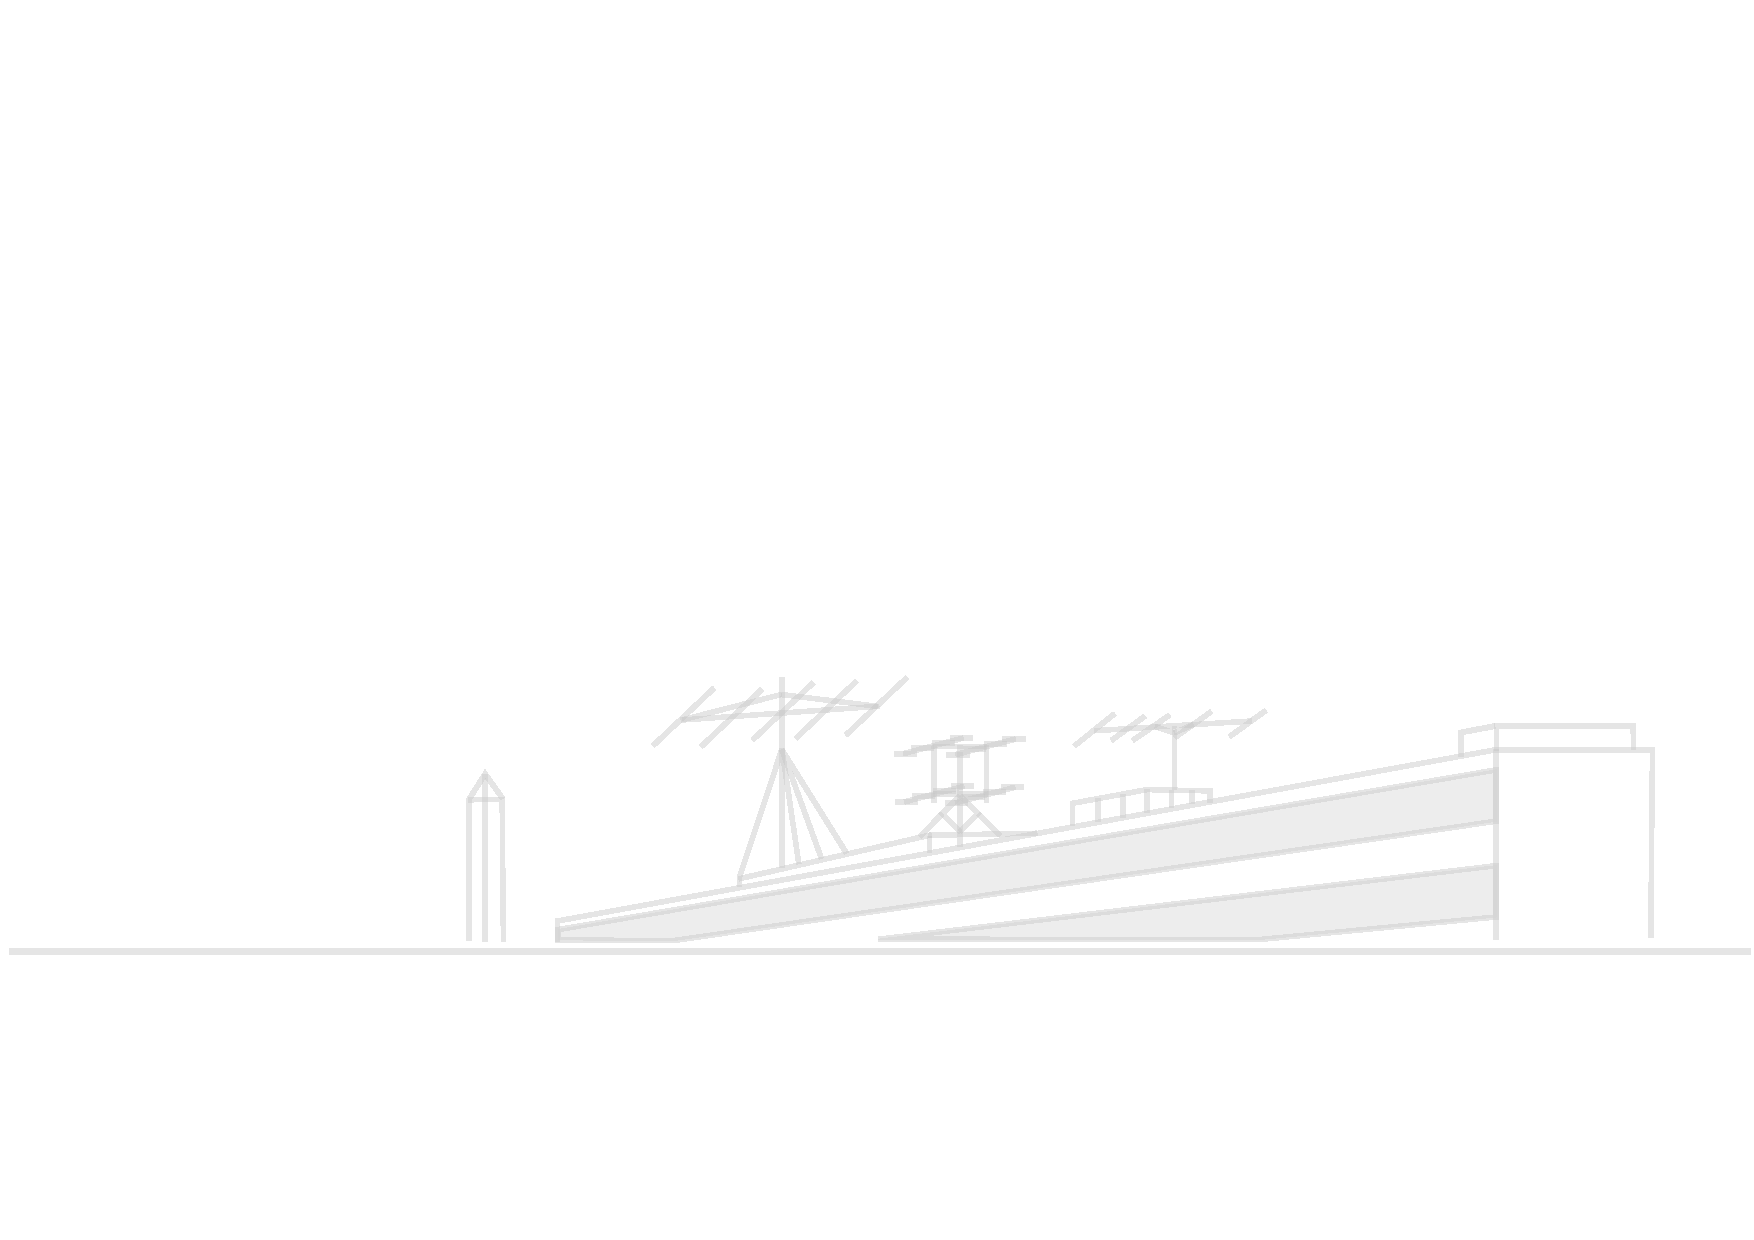
\includegraphics[width=17.8cm]{texdata/dk0tu_rooftop_background.pdf}
}

% Foliennummer einfügen
\setbeamertemplate{footline}[frame number]
%\setbeamertemplate{footline}{}

% Ändere das Zeichen vor jedem item
%\setbeamertemplate{itemize item}{\color{craneorange}$\blacktriangleright$}
%\setbeamertemplate{itemize subitem}{\color{craneorange}$\triangleright$}
%\setbeamertemplate{itemize subsubitem}{\color{craneorange}$\blacktriangleright$}

% Ändert die Blöcke 
\setbeamertemplate{blocks}[rounded][shadow=true]
% default | rounded [shadow=true|false]

%
% Eigene Kommandos
%

% Hack to get natbib and beamer working together. "The beamer user guide suggests
% that only the manual bibliography entry approach is supported"
% on some system it works out of the box, sometimes you need the hack :-(
% so check it --dl7bst
\ifdefined\newblock
    \relax
\else
    \newcommand{\newblock}{}
\fi

% \includedia command to generate png out of a dia file
% NEEDS installed dia and pdflatex option --shell-escape
\newcommand{\includedia}[1]{
    \immediate\write18{/usr/bin/dia #1.dia -e #1_diatmp.png -t png}
}

% RICHIG GROSSER FONT!
\newfont{\bigfont}{cmr10 at 144pt}
\newfont{\smallfont}{cmr10 at 8pt}

% Römische Ziffern
\makeatletter
\newcommand{\rmnum}[1]{\romannumeral #1}
\newcommand{\Rmnum}[1]{\expandafter\@slowromancap\romannumeral #1@}
\makeatother

% Schwarze Überschrift
%\setbeamercolor{frametitle}{fg=black}
%\setbeamercolor{title}{fg=black}

% Item- und Box-Farben
\definecolor{deepBlue}{HTML}{000066}
\setbeamercolor{itemize item}{fg=deepBlue}
\setbeamercolor{itemize subitem}{fg=deepBlue}
\setbeamercolor{description item}{fg=deepBlue}
\setbeamercolor{block title}{fg=deepBlue!100, bg=blue!15}
\setbeamercolor{block body}{fg=black, bg=blue!5}
\setbeamercolor{block title alerted}{fg=deepBlue, bg=red!75}
\setbeamercolor{block body alerted}{fg=black, bg=red!15}
\setbeamercolor*{block title example}{fg=blue!50, bg=blue!10}
\setbeamercolor*{block body example}{fg= blue, bg=blue!5}

%\setbeamercolor{section in head/foot}{parent=palette primary}
%\setbeamercolor{subsection in head/foot}{parent=palette secondary}
%\setbeamercolor{sidebar}{fg=darkblue,bg=yellow!90!orange}
%\setbeamercolor{title in sidebar}{fg=darkblue}
%\setbeamercolor{author in sidebar}{fg=darkblue}
%\setbeamercolor{section in sidebar}{fg=darkblue!10!black}
%\setbeamercolor{subsection in sidebar}{fg=darkblue!50!black}

% Titlepage Infos
\title{AFu-Kurs nach DJ4UF}
\author[DKØTU]{DKØTU\\ \footnotesize{Amateurfunkgruppe der TU Berlin}}
\institute[DKØTU]{\url{http://www.dk0tu.de} }

% PDF-Eigenschaften
\subject{DK0TU-Amateurfunkkurs nach DJ4UF}
\keywords{Amateurfunk Kurs HAM Radio Course CC-BY-NC-SA OpenSource TU Berlin DK0TU}

\subtitle{Betriebstechnik/Vorschriften 11: \\
Betriebsabwicklung auf VHF/UHF \\[2em]}
\date{Stand 18.09.2017}
 \begin{document}

\begin{frame}
    \titlepage
    \vfill
    \begin{center}
        \ccbyncsaeu\\
        {\tiny This work is licensed under the \em{Creative Commons Attribution-NonCommercial-ShareAlike 3.0 License}.}\\[0.5ex]
         \tiny Amateurfunkgruppe der Technische Universität Berlin (AfuTUB), DKØTU
         %\includegraphics[scale=0.5]{img/DK0TU_Logo.pdf}
    \end{center}
\end{frame}


%FIXME Quellen aus den Slides ins Verzeichnis
%TODO Reihenfolge Moltrecht angelehnt - ist aber Quark, z.B. Locator weit vorziehen
%TODO Quellen in den Fußnoten nehmen zu viel Platz weg -> Anhang

\section*{Einleitung}

\begin{frame}
  \frametitle{Einleitung}

  \begin{block}{Von welchen Frequenzbereichen reden wir bei VHF und UHF?}
    \only<1>{\vspace{1em}}
    \only<2>{Richtig, $30-300MHz$ (VHF) und $300-3000MHz$ (UHF)}
  \end{block}

\end{frame}

\section[UKW]{UKW-Eigenschaften}

\begin{frame}
  \frametitle{UKW-Eigenschaften}

  \begin{itemize}
    \item Freiraumausbreitung, eine quasi-optische Ausbreitung, ähnlich dem
      Licht
    \item Reichweite normalerweise ca. 10 bis 250km -- was sind die Faktoren?

      \pause

      \begin{itemize}
        \item Frequenzbereich
        \item Gelände
        \item Antennenhöhe
        \item Sendeleistung
        \item Betriebsart
        \item abwarten... Überreichweiten bis über 2000km
      \end{itemize}
  \end{itemize}

\end{frame}

\section[Verkehrsarten]{Verkehrs- bzw. Verbindungsarten in der Nachrichtentechnik}

\subsection{SX}

\begin{frame}
  \frametitle{Simplex (SX)}

  SX, auch \emph{Richtungsverkehr}, eigentlich reine
  ``one-way''-Kommunikation: Daten können in nur eine Richtung übertragen
  werden, diese Technik ermöglicht keine Antwort.

  \begin{center}
    \begin{figure}
      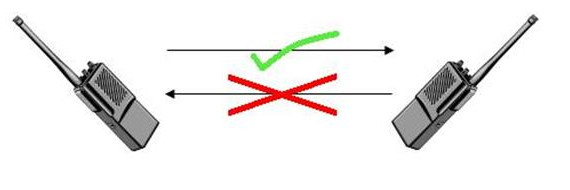
\includegraphics[width=0.6\textwidth]{bv11/Simplex.jpg}
      \attribcaption{Simplex}{SImedioP}{http://commons.wikimedia.org/wiki/File:Simplex.jpg}{\ccbysa}
    \end{figure}
  \end{center}

  \begin{itemize}
    \item Beispiele:
      \begin{itemize}
        \item Broadcast: Hörfunk, Fernsehen, Funk-Baken, GPS, ...
        \item Funkmikro, Babyfon
        \item Pager
      \end{itemize}
  \end{itemize}

\end{frame}

\subsection{HX}

\begin{frame}
  \frametitle{Halbduplex (HX)}

  Beim Halb- oder Semiduplex, auch \emph{Wechselverkehr} oder \emph{Bedingter
  Gegenverkehr} können Daten abwechselnd, aber nicht gleichzeitig, in beide
  Richtungen fließen.

  \begin{center}
    \begin{figure}
      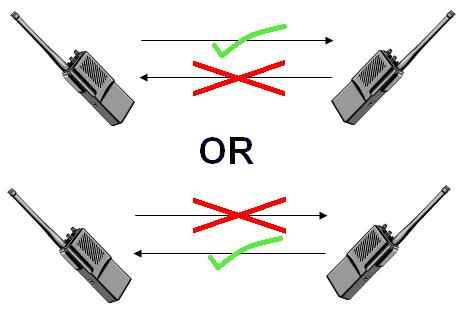
\includegraphics[width=0.6\textwidth,height=.6\textheight,keepaspectratio]{bv11/HalfDuplex.jpg}
      \attribcaption{Half Duplex}{Greggreggreg}{http://commons.wikimedia.org/wiki/File:HalfDuplex.JPG}{\ccpd}
    \end{figure}
  \end{center}

\end{frame}

\begin{frame}
  \frametitle{Halbduplex (HX)}

  \begin{itemize}
    \item Simplex ITU-T definition: One way signaling at a time
    \item SX im AFu oft auch stellvertretend für Kommunikation, die nur eine Frequenz
      zum Senden und Empfangen nutzt, anstatt einen Repeater zu nutzen
    \item gemeint ist aber Halbduplex bzw. Semiduplex
  \end{itemize}

  \begin{columns}
    \column{.6\textwidth}
      \begin{itemize}
        \item zum Vergleich:
          \begin{itemize}
            \item AFu-Handfunkbetrieb
            \item Intercom/Türsprechanlage
            \item CB-Funk
            \item PMR-Funk
          \end{itemize}
      \end{itemize}

    \column{.4\textwidth}
    \begin{center}
      \begin{figure}
        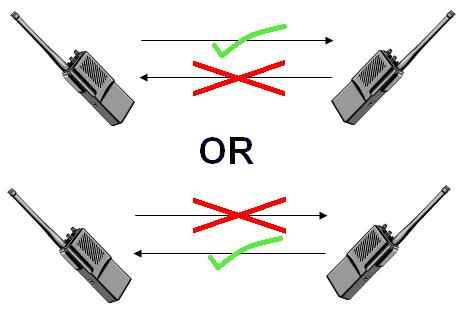
\includegraphics[width=\textwidth,height=.4\textheight,keepaspectratio]{bv11/HalfDuplex.jpg}
        \attribcaption{Half Duplex}{Greggreggreg}{http://commons.wikimedia.org/wiki/File:HalfDuplex.JPG}{\ccpd}
      \end{figure}
    \end{center}
  \end{columns}

\end{frame}

\subsection{DX}

\begin{frame}
  \frametitle{Vollduplex (DX)}

  Beim DX\footnote{nicht verwechseln mit weite Entfernung}, auch
  \emph{Gegenverkehr}, können Daten in beide Richtungen gleichzeitig
  übertragen werden. \\[1em]

  \begin{center}
    \begin{figure}
      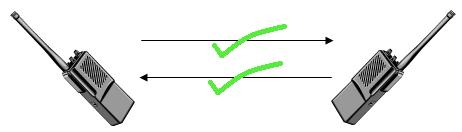
\includegraphics[width=0.6\textwidth,height=.25\textheight,keepaspectratio]{bv11/FullDuplex.jpg}
      \attribcaption{Full Duplex}{Greggreggreg}{http://commons.wikimedia.org/wiki/File:FullDuplex.JPG}{\ccpd}
    \end{figure}
  \end{center}

  \begin{itemize}
    \item Beispiele:

      \begin{itemize}
        \item Telefon
        \item Ethernet
        \item ``Datenfunk'' via Satelliten oder HamNet
      \end{itemize}
  \end{itemize}

\end{frame}

\section[FM-Funkbetrieb]{Einfacher FM-Funkbetrieb}

\begin{frame}
  \frametitle{Einfacher FM-Funkbetrieb}

  In den so genannten Simplex-Bereichen\footnote{NBFM (Narrow-Band FM) mit ca. 12~kHz
  Bandbreite, Kanalraster 12,5~kHz} finden lokale ``Runden'' statt.
  Ein \emph{QSO} startet z.B. mit: \\[2em]

  \begin{center}
    \Large \emph{``[Hier ist ein] Allgemeiner Anruf von DKØTU''} \\[1em]
    \normalsize oder \\[1em]
    \Large \emph{``[CQ] DKØTU von DL7BST''}
  \end{center}

\end{frame}

\begin{frame}
  \frametitle{Einfacher FM-Funkbetrieb}

  \begin{itemize}
    \item es folgen so genannte Durchgänge in die man sich reinhängen kann --
      nicht brachial, sondern vorsichtig
    \item lockere Gesprächsathmosphäre ohne Q-Codes
    \item mitschreiben der Gegenstationen und ihre Rapporte hilft
    \item QTH nennen, Rig vorstellen
    \item außerhalb von Runden freie QRG suchen oder entsprechende
      Anruffrequenz nutzen
  \end{itemize}

\end{frame}

\subsection{Relaisbetrieb}

\begin{frame}
  \frametitle{Relaisbetrieb}

  \begin{center}
    \begin{figure}
      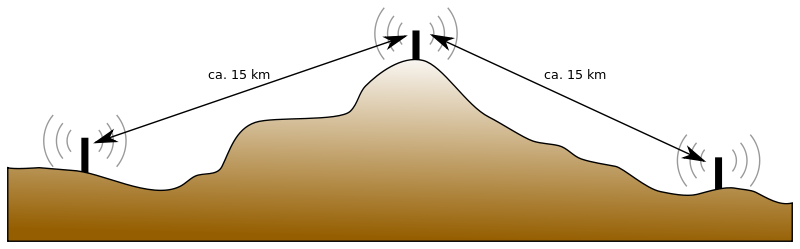
\includegraphics[width=1\textwidth,height=.6\textheight,keepaspectratio]{bv11/Relaisstelle.png}
      \attribcaption{Relaisstelle}{$\aleph$ (Aleph)}{http://commons.wikimedia.org/wiki/File:Relaisstelle.svg}{Beerware Licence}
    \end{figure}
  \end{center}

  \begin{itemize}
    \item Umsetzerstationen, normalerweise exponiert -- warum?
    \item unterschiedliche Ein-/Ausgabe-Frequenz im gleichen Band (Duplex)
  \end{itemize}

\end{frame}

\begin{frame}
  \frametitle{Relaisfunkbetrieb}

  \begin{center}
    \begin{figure}
      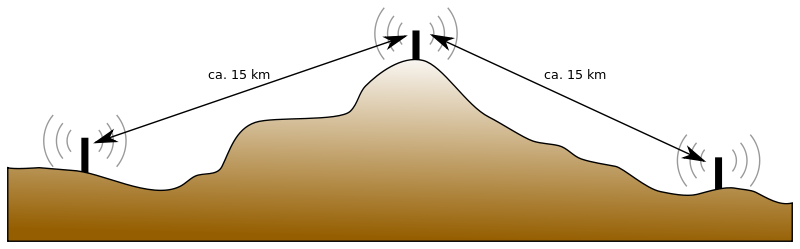
\includegraphics[width=0.5\textwidth,height=.3\textheight,keepaspectratio]{bv11/Relaisstelle.png}
      \attribcaption{Relaisstelle}{$\aleph$ (Aleph)}{http://commons.wikimedia.org/wiki/File:Relaisstelle.svg}{Beerware Licence}
    \end{figure}
  \end{center}

  \begin{itemize}
    \item QRGs werden abgestimmt und bei \emph{BNetzA} angemeldet
    \item Ablage oder Shift (abweichend in anderen Ländern):
      \begin{itemize}
        \item 2-m-Band: $600 kHz$
        \item 70-cm-Band: $7,6 MHz$
        \item 23-cm-Band: $35 MHz$
        \item MERKE: Das Relais sendet ``von oben''!
      \end{itemize}
    \item Öffnung meist mit 1750-Hz-Ton -- bei Erfolg hört man die Kennung
    \item manche Relais verwenden CTCSS/DTS
  \end{itemize}

\end{frame}

\subsection{Echolink}

\begin{frame}
  \frametitle{Echolink}

  Betriebsart, die Repeater über das Internet verbindet.

  \begin{center}
    \begin{figure}
      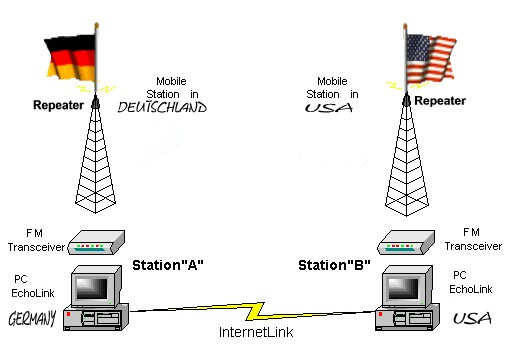
\includegraphics[width=0.6\textwidth,height=.45\textheight,keepaspectratio]{bv11/Echolink.jpg}
      \attribcaption{Echolink}{Stahlecker}{http://commons.wikimedia.org/wiki/File:Echolink.jpg}{Copyrighted free use}
    \end{figure}
  \end{center}

  \begin{itemize}
    \item Ziel-Knotennummern können mit DTMF\footnote{Dual-tone multi-frequency
      (Mehrfrequenzwahlverfahren)}-Tönen gewählt werden
    \item außer zusätzliches Delay kaum Unterschied zum Relais
  \end{itemize}

\end{frame}

\section[Ausbreitungsbed.]{Besondere Ausbreitungsbedingungen}

\subsection[Tropo DX]{Troposphärische Überreichweiten (Tropo DX)}

\begin{frame}
  \frametitle{Troposphärische Überreichweiten (Tropo DX)}

  \begin{center}
    \begin{figure}
      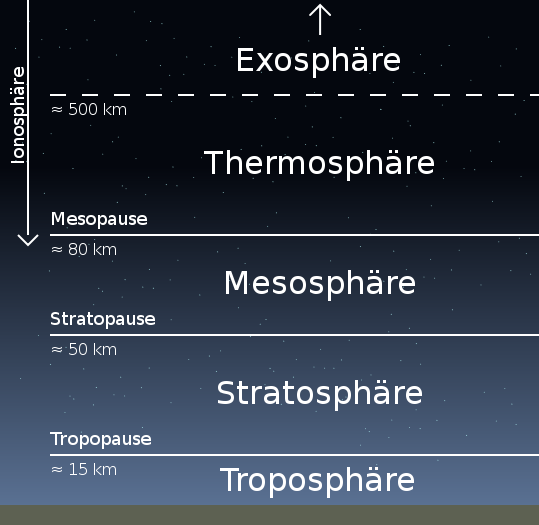
\includegraphics[width=0.5\textwidth,height=.6\textheight,keepaspectratio]{bv11/Atmosphaere_Stufen.png}
      \attribcaption{Atmosphäre Stufen}{Niko Lang (original image), Ladyt (vector version)}{http://commons.wikimedia.org/wiki/File:Atmosphäre_Stufen.svg}{\ccbysa}
    \end{figure}
  \end{center}

  Troposphäre: Unterste Schicht der Erdatmosphäre AKA \emph{Wetterschicht}

\end{frame}

\begin{frame}
  \frametitle{Troposphärische Überreichweiten (Tropo DX)}

  \begin{center}
    \begin{figure}
      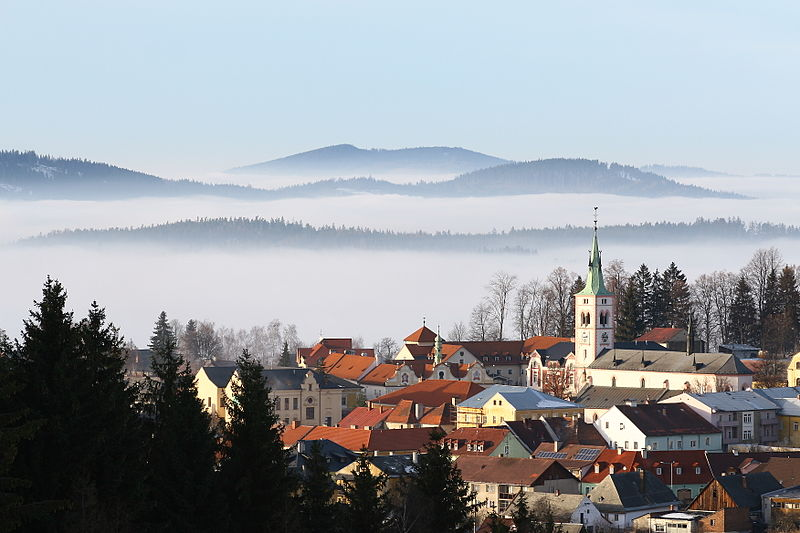
\includegraphics[width=0.6\textwidth,height=.5\textheight,keepaspectratio]{bv11/Inversionswetterlage.jpg}
      \attribcaption{Inversionswetterlage}{Adam Hauner}{https://commons.wikimedia.org/wiki/File:Kašperské Hory od Liščího vrchu.jpg}{\ccby}
    \end{figure}
  \end{center}

  \begin{itemize}
    \item größter Teil der Wärme wird vom Erdboden aufgenommen, weswegen die
      Lufttemperatur im Schnitt um etwa 6,5$^\circ$C pro Kilometer Höhe abnimmt
    \item Metereologische Vorgänge können für Inversionen sorgen
  \end{itemize}

\end{frame}

\begin{frame}
  \frametitle{Troposphärische Überreichweiten (Tropo DX)}

  \begin{columns}
    \column{.5\textwidth}
      \begin{center}
        \begin{figure}
          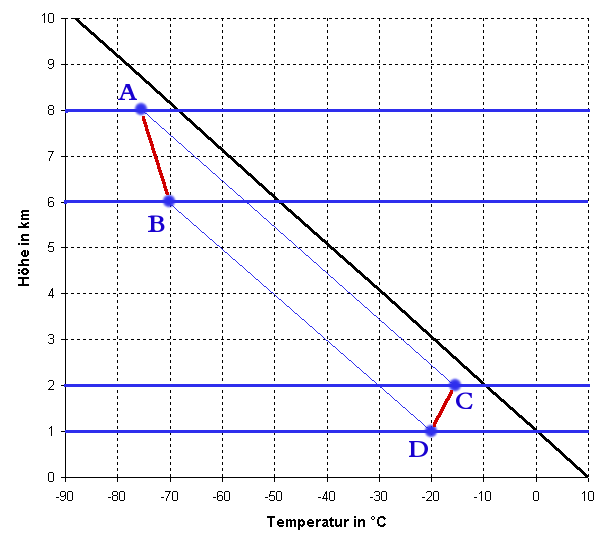
\includegraphics[width=\textwidth,height=.8\textheight,keepaspectratio]{bv11/Absinkinversion.png}
          \attribcaption{Absinkinversion}{Saperaud}{http://commons.wikimedia.org/wiki/File:Absinkinversion.png}{\ccpd}
        \end{figure}
      \end{center}
    \column{.5\textwidth}
      \begin{itemize}
        \item an den Sprüngen kann UKW gebrochen werden, 100 bis 1000km Reichweite
        \item meist Herbst und Frühling
        \item kurze Durchgänge: Rapport, Locator und eventuell noch Namen
        \item Beispiel: QSO zwischen DC4LW in Berlin und DO1DAN mit 10W in Dannenberg (200km) via DB0BLO (70cm) an einem Septembermorgen
      \end{itemize}
\end{columns}

\end{frame}

\subsection{Aurora borealis}

\begin{frame}
  \frametitle{Aurora borealis}

  \begin{center}
    \begin{figure}
      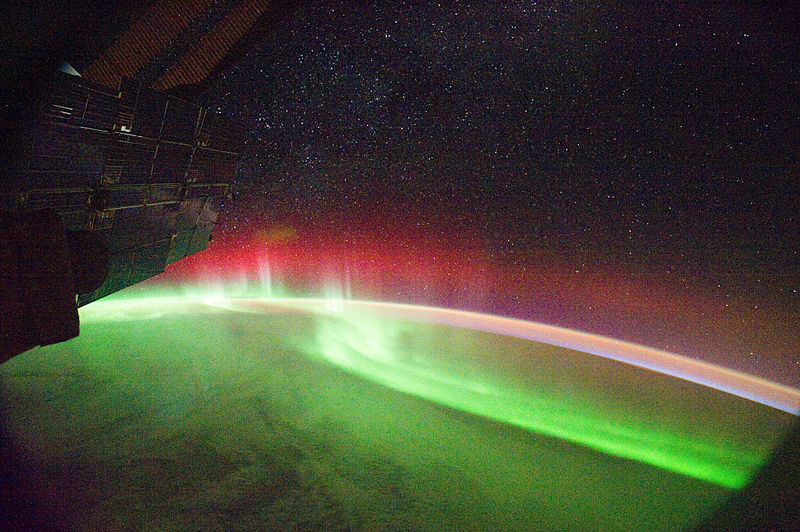
\includegraphics[width=0.6\textwidth,height=.5\textheight,keepaspectratio]{bv11/Aurora_Seen_From_Space_by_NASA.jpg}
      \attribcaption{Aurora Seen from Space by NASA}{NASA}{http://commons.wikimedia.org/wiki/File:Aurora_Seen_From_Space_by_NASA.jpg}{\ccpd}
    \end{figure}
  \end{center}

  Um das Sonnenfleckenmaximum (ca. 11-Jahres-Zyklus) herum gibt es starke
  Sonnenwinde als kurzzeitige Erscheinungen.

  \begin{itemize}
    \item Erdmagnetfeld zieht diese auf die Polkappen, ionisiert diese (Polarlicht).
  \end{itemize}

\end{frame}

\begin{frame}
  \frametitle{Aurora borealis}

  \begin{center}
    \begin{figure}
      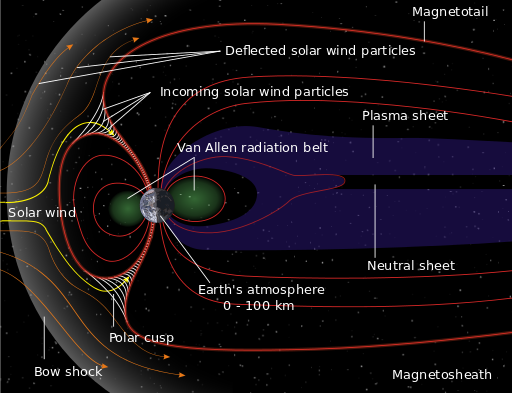
\includegraphics[width=0.6\textwidth,height=.5\textheight,keepaspectratio]{bv11/Structure_of_the_magnetosphere-en.png}
      \attribcaption{Structure of the Magnetosphere}{Original bitmap from NASA. SVG rendering by Aaron Kaase}{http://commons.wikimedia.org/wiki/File:Structure_of_the_magnetosphere-en.svg}{\ccpd}
    \end{figure}
  \end{center}

  \begin{itemize}
    \item VHF wird stark verzerrt (verrauscht und verbrummt) reflektiert
    \item kein SSB/FM, nur Telegrafie
    \item Antennenrichtung: Null +/- 30 Grad
  \end{itemize}

\end{frame}

\subsection{Sporadic-E}

\begin{frame}
  \frametitle{Sporadic-E}
  \begin{columns}
    \column{.4\textwidth}
      \begin{center}
        \begin{figure}
          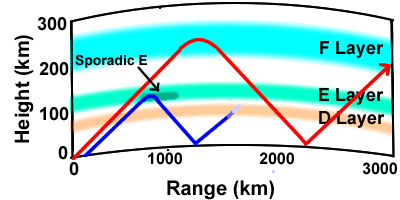
\includegraphics[width=\textwidth,height=.85\textheight,keepaspectratio]{bv11/SporadicE-NPS.png}
          \attribcaption{Sporadic E. {\color{red} Rot: Normale KW} {\color{blue} Blau: KW bei Sporadic E}}{Naval Postgraduate School}{http://commons.wikimedia.org/wiki/File:SporadicE-NPS.gif}{\ccpd}
        \end{figure}
      \end{center}
    \column{.6\textwidth}
      $E_S$-Schicht: In Frühsommermonaten sporadisch stark ionisierte Bereiche am
      unteren Rand der E-Schicht.

      \begin{itemize}
        \item Entstehung ist nicht geklärt
        \item Bei KW Ausbreitung und Empfang der “toten Zone” möglich, aber kein DX
        \item Aber auch UKW wird gebrochen $\rightarrow$ Reichweitensteigerung
        \item 1000 bis 2000km Hops mit QRP
        \item keine stetige Verbindung, Schichten ändern sich innerhalb weniger Minuten
        \item kurze Durchgänge: Rapport, Locator und eventuell noch Namen
      \end{itemize}
  \end{columns}
\end{frame}

\begin{frame}
  \frametitle{Vergleich der Überreichweiten}

  \begin{center}
    \begin{figure}
      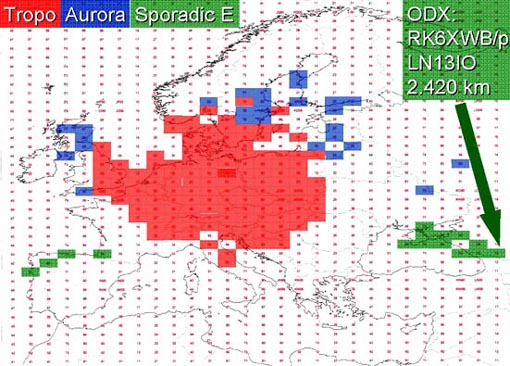
\includegraphics[width=0.9\textwidth,height=.65\textheight,keepaspectratio]{bv11/df0yy_2m-karte.jpg}
      \attribcaption{2m Karte bei Überreichweiten}{DFØYY}{http://www.df0yy.de/workingus.htm}{}
    \end{figure}

    Gearbeitete Großfelder von \emph{DFØYY} auf dem 2 Meter Band
  \end{center}

\end{frame}

\subsection[Meteorscatter]{Meteorscatter (MS)}

\begin{frame}
  \frametitle{Meteorscatter (MS)}

  In die Atmosphäre eintretende Meteoritenschauer ionisieren die
  Luftschichten.

  \begin{columns}
    \column{.4\textwidth}
      \begin{center}
        \begin{figure}
          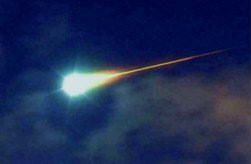
\includegraphics[width=\textwidth,height=.85\textheight,keepaspectratio]{bv11/Bolide.jpg}
          \attribcaption{Meteor}{Thomas Grau derivative work: Basilicofresco}{http://commons.wikimedia.org/wiki/File:Bolide.jpg}{\ccpd}
        \end{figure}
      \end{center}
    \column{.6\textwidth}
      \begin{itemize}
        \item ca. 100 km Höhe
        \item Sekundenbruchteile (Ping), wenige Sekunden (Burst), sehr selten
          mehrere Minuten
        \item Hops von ca. 800 bis 2500 km
        \item High-Speed-Telegrafie (Computer- bzw. Tonbandgestützt) oder Digimodes wie FSK441
        \item extrem verkürzte SSB-Kontakte selten möglich
      \end{itemize}
  \end{columns}

  %todo Der Pro schaut sich das mal an: "Determining the radiant of a meteor"
  %     http://ea4eoz.blogspot.com.es/2015/05/determining-radiant-of-meteor-using.html

\end{frame}

\subsection[EME]{Erde-Mond-Erde (EME)}

\begin{frame}
  \frametitle{Erde-Mond-Erde (EME)}

  Mondoberfläche als Reflektor für UKW

  \begin{columns}
    \column{.5\textwidth}
      \begin{center}
        \begin{figure}
          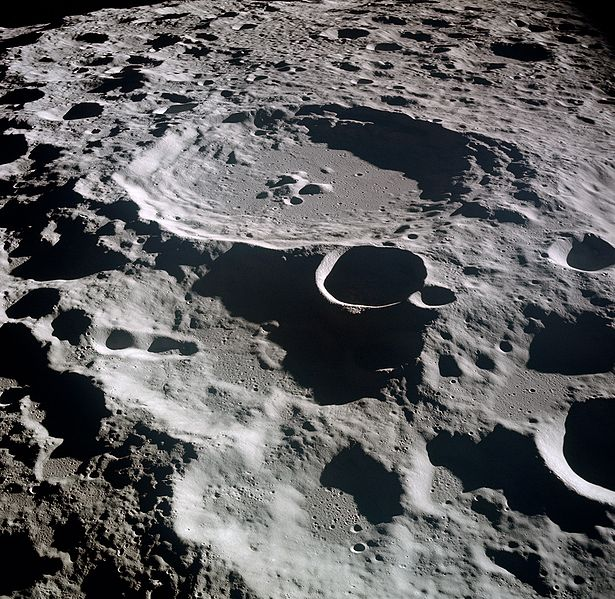
\includegraphics[width=\textwidth,height=.7\textheight,keepaspectratio]{bv11/Lunar_crater_Daedalus.jpg}
          \attribcaption{Lunar Crater Daedalus}{NASA}{http://commons.wikimedia.org/wiki/File:Lunar_crater_Daedalus.jpg}{\ccpd}
        \end{figure}
      \end{center}
    \column{.5\textwidth}
      \begin{itemize}
        % Die Angabe º ist korrekt, da hier die Größe am Himmel angegeben wird
        \item Mond ca. 0,5º der Himmelsoberfläche
        \item vom Mond aus Erde auch nur ca. 2º
        \item extrem schlechter Reflektor (10\%, diffus), 250dB Dämpfung bei 2m-Band
        \item ergo: gute Richtwirkung, QRO und Schmalbandbetriebsarten (CW, Digimodes wie JT65)
      \end{itemize}
  \end{columns}

\end{frame}

\begin{frame}
  \begin{center}
    \begin{figure}
      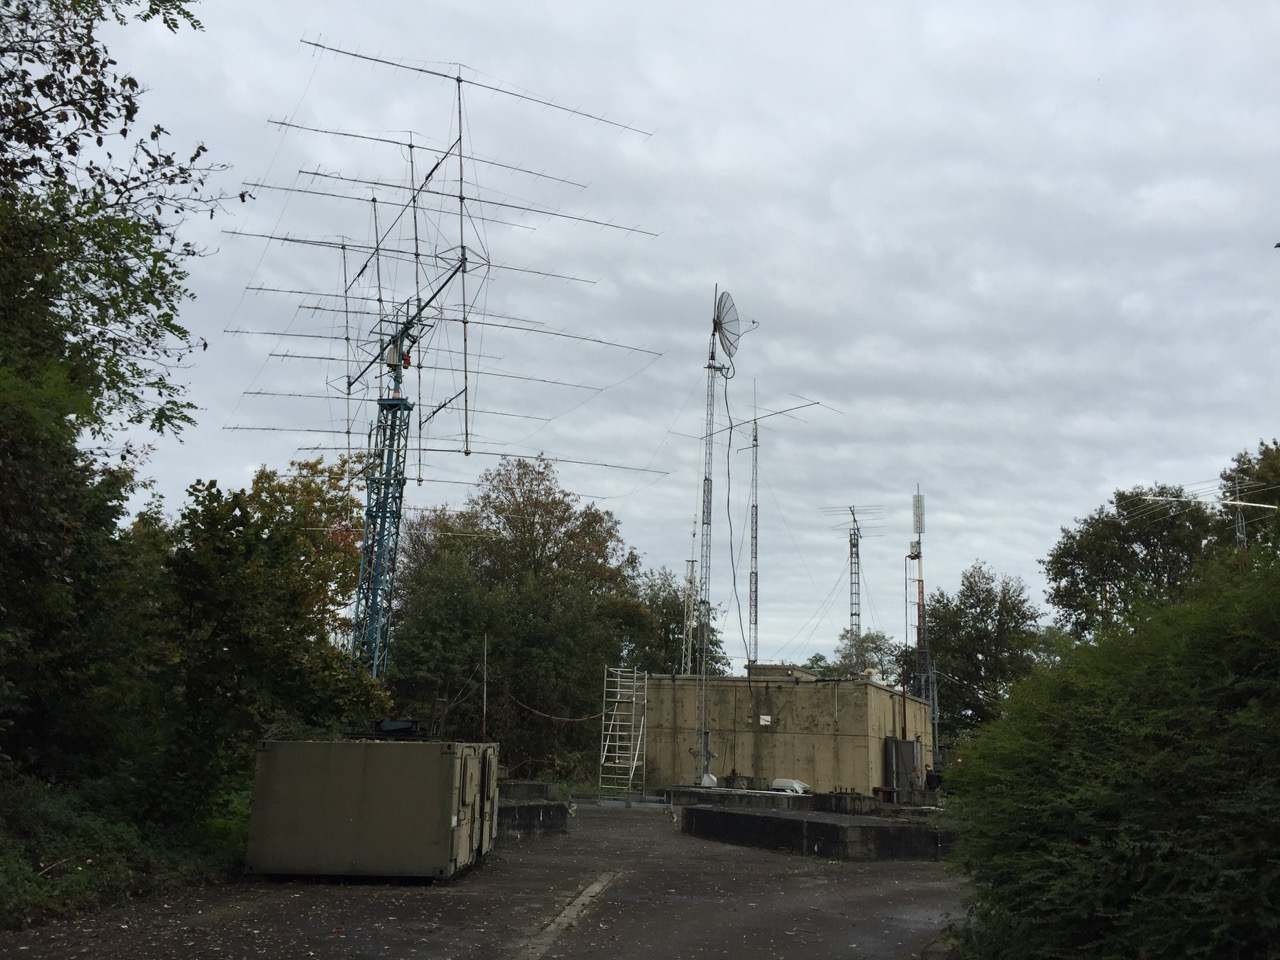
\includegraphics[width=1\textwidth,height=.9\textheight,keepaspectratio]{bv11/IMG_2898.jpg}
      \attribcaption{DFØMU in Schöppingen}{DC4LW}{http://dc4lw.de}{}
    \end{figure}
  \end{center}
\end{frame}

\begin{frame}
  \begin{center}
    \begin{figure}
      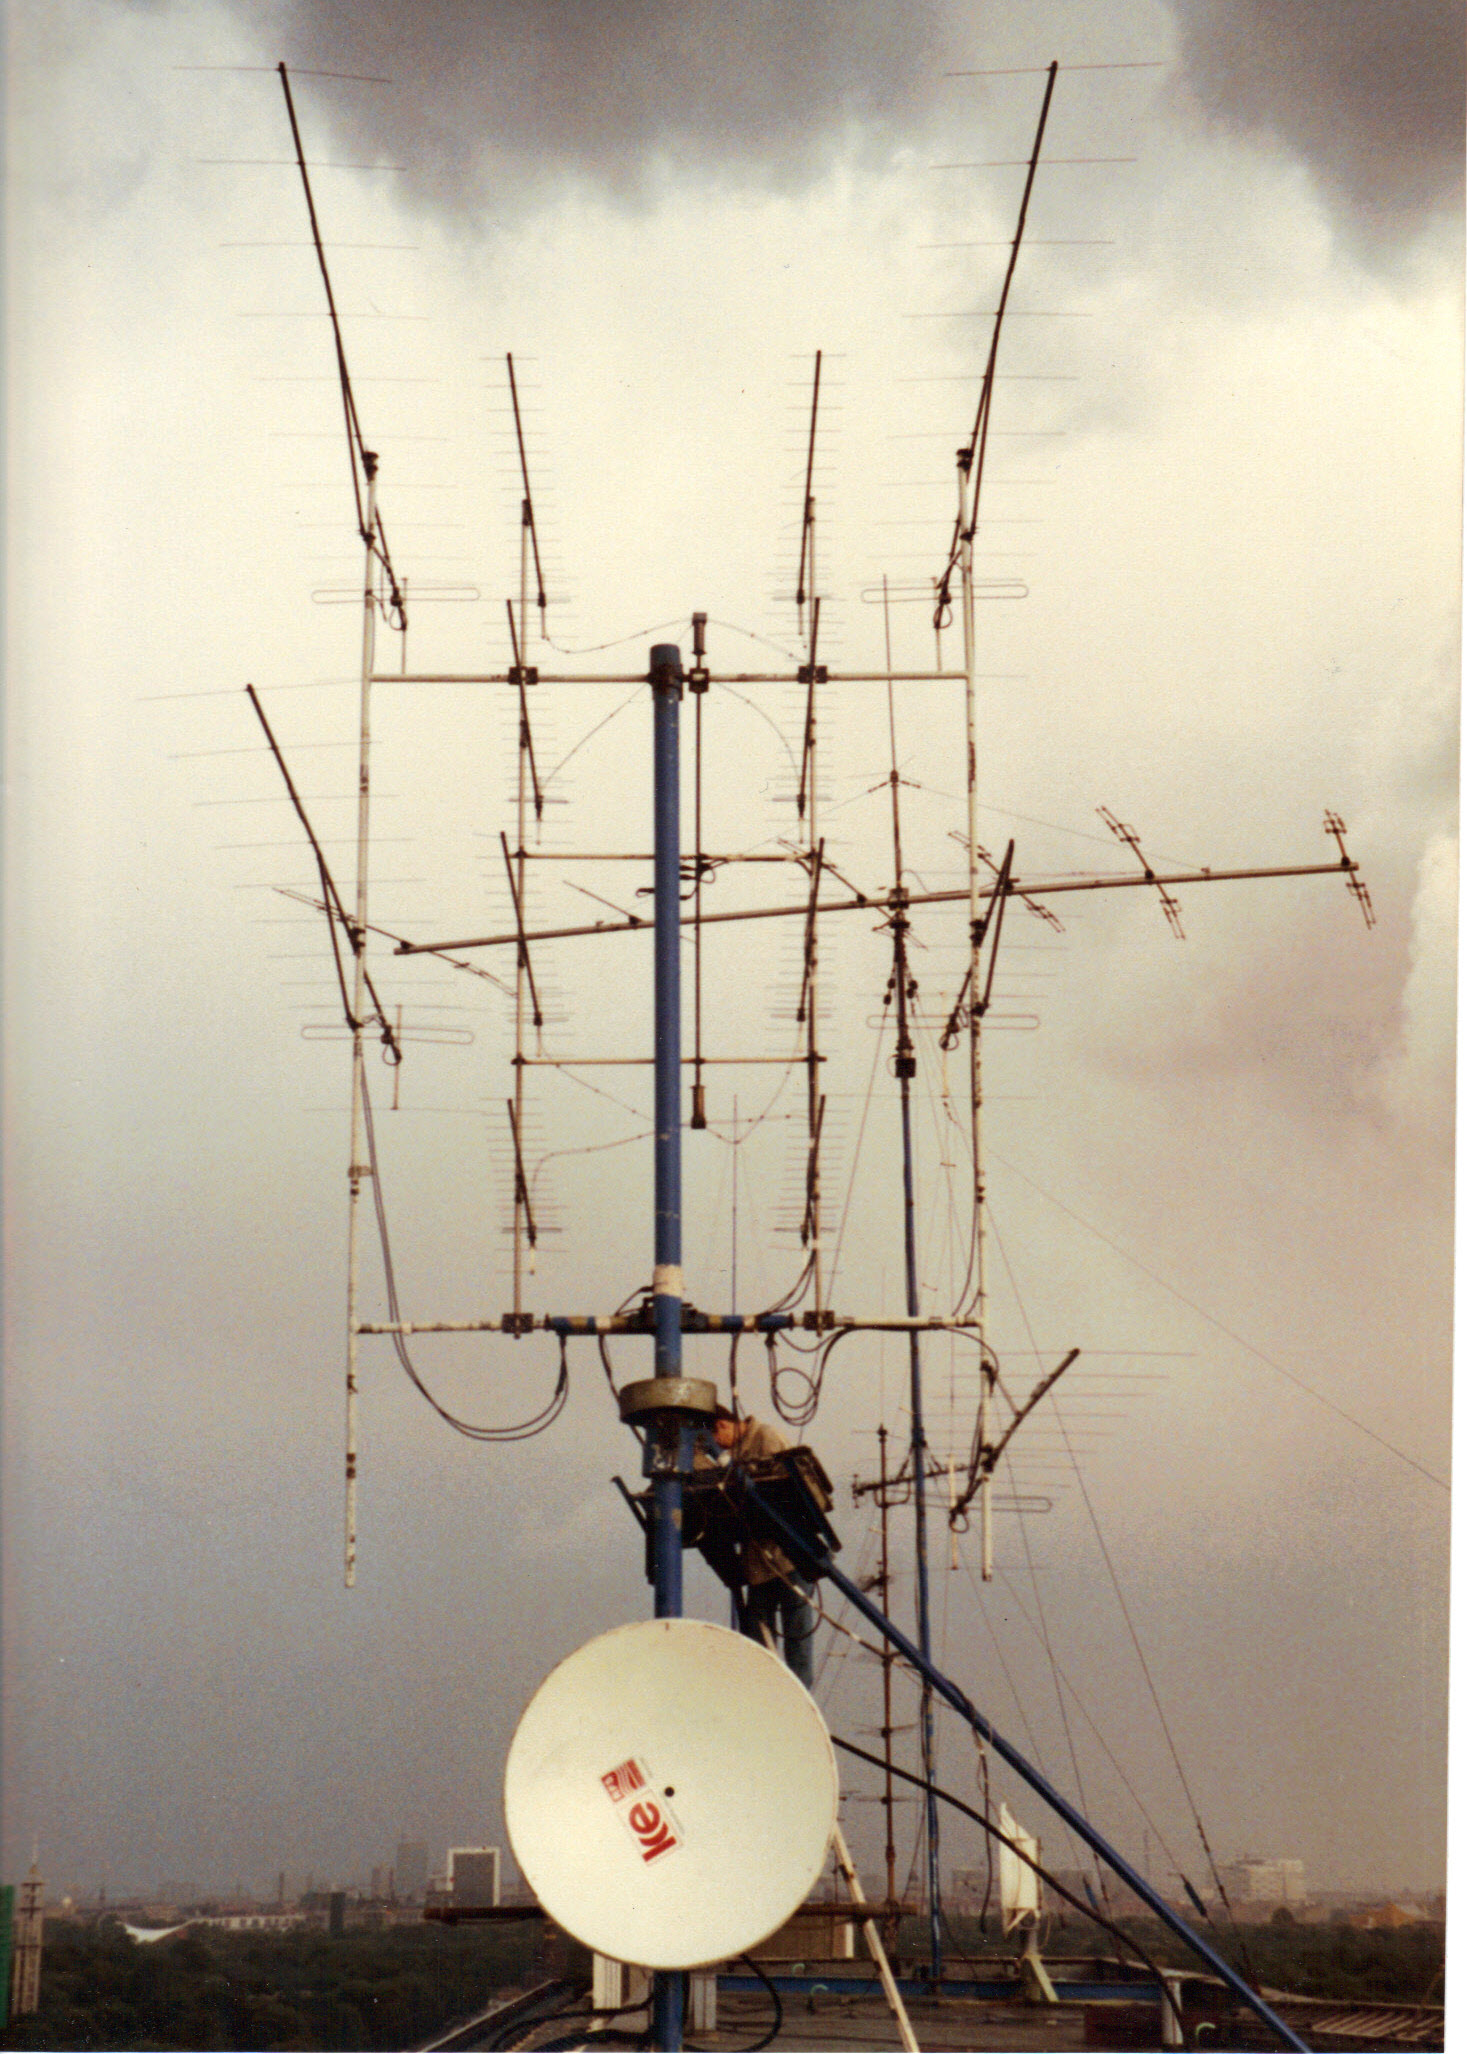
\includegraphics[width=1\textwidth,height=.9\textheight,keepaspectratio]{bv11/1988+89_UKW-Gruppen_G8VHI.jpg}
      \attribcaption{UKW-Gruppen bei DKØTU im Jahr 1988/89}{DKØTU}{http://www.dk0tu.de/chronicle/1988+89_UKW-Gruppen_G8VHI.jpg}{}
    \end{figure}
  \end{center}
\end{frame}

\section{Transponder}

\begin{frame}
  \frametitle{Transponder}

  Kofferwort aus Transmitter und Responder -- im Prinzip ein Breitbandrelais.

  \begin{center}
    \begin{figure}
      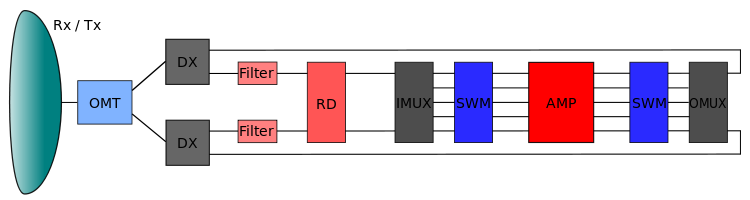
\includegraphics[width=0.5\textwidth,height=.3\textheight,keepaspectratio]{bv11/Transponder.png}
      \attribcaption{Transponder}{Dantor}{http://commons.wikimedia.org/wiki/File:Transponderp.svg}{\ccbysa}
    \end{figure}
  \end{center}

  \begin{itemize}
    \item Meist sind Lineartransponder gemeint, die einen Frequenzbereich
      duplex auf einen anderen umsetzen -- unabhängig von der Betriebsart
    \item oftmals verschiedene Bänder
    \item RX, Amplify, TX
    \item geringe Leistung verwenden, da \emph{AGC} nach stärkstem Signal regelt
    \item einige Transponder können diese \emph{Krokodile} ausnotchen
  \end{itemize}

\end{frame}

\subsection{ARTOB}

\begin{frame}
  \frametitle{ARTOB}

  \textbf{A}mateur \textbf{R}adio \textbf{T}ransponder \textbf{O}n \textbf{B}aloon

  \begin{center}
    \begin{figure}
      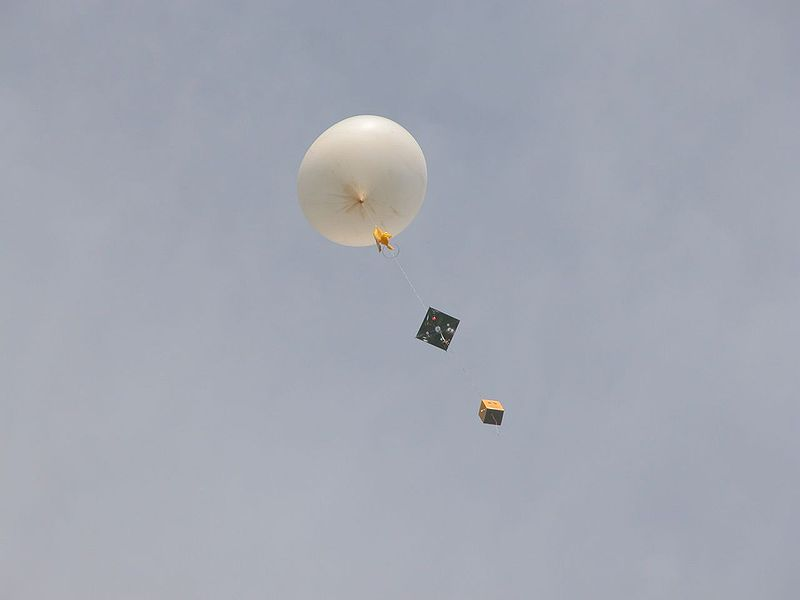
\includegraphics[width=0.6\textwidth,height=.5\textheight,keepaspectratio]{bv11/Wetterballon_Nutzlast.jpg}
      \attribcaption{Wetterballon Nutzlast}{Harald Linden O28 Lennestadt}{https://commons.wikimedia.org/wiki/File:Wetterballon_Nutzlast_Start_2004-09-10.jpg}{GPL}
    \end{figure}
  \end{center}

  \begin{itemize}
    \item Möglichkeit einen Transponder für günstige Ausbreitung zu nutzen
    \item Höhe bis zu 30 km
  \end{itemize}

  % www.aatis.org

\end{frame}

\subsection{OSCAR}

\begin{frame}
  \frametitle{OSCAR}

  %todo Geschichte, Fotos, Videos?

  \textbf{O}rbiting \textbf{S}atellite \textbf{C}arrying \textbf{A}mateur \textbf{R}adio

  \begin{center}
    \begin{figure}
      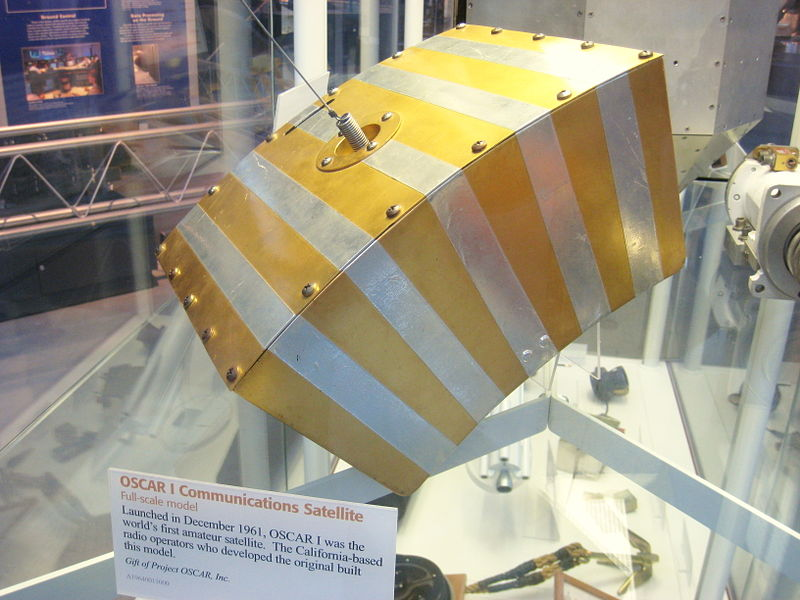
\includegraphics[width=0.6\textwidth,height=.5\textheight,keepaspectratio]{bv11/OSCAR1.jpg}
      \attribcaption{OSCAR1}{Daderot}{https://commons.wikimedia.org/wiki/File:OSCAR_1_Communications_Satellite_model_-_Udvar-Hazy_Center.JPG}{\ccpd}
    \end{figure}
  \end{center}

  \begin{itemize}
    \item Satellitenfunkbetrieb
    \item bereits 12/1961 \emph{OSCAR 1} (vgl. \emph{Sputnik 1} 10/1957)
  \end{itemize}

\end{frame}

\begin{frame}
  \frametitle{OSCAR}

  \begin{itemize}
    \item meist auf elliptische Umlaufbahnen, Parameter:
      \begin{itemize}
        \item Azimut
        \item Elevation
        \item Apogäum (max. Entfernung)
        \item Perigäum (min. Entf.)
      \end{itemize}
    \item Up- und Downlink\footnote{2-m-Band: 145,300-146,500 MHz; 70-cm-Band: 438,000-440,000 MHz}
      oft in verschiedenen Bändern (Transponderfahrplan)
    \item teilweise SSB mit LSB im Uplink und USB im Downlink
    \item old and busted coming up: geostationär (35.786 km)
    \item new hotness coming up: Kleinsatelliten (CubeSat und kleiner)
  \end{itemize}

\end{frame}

\section[QTH-Locator]{QTH-Locator (Maidenhead Locator)}

\begin{frame}
  \frametitle{QTH-Locator (Maidenhead Locator)}

  \begin{center}
    \begin{figure}
      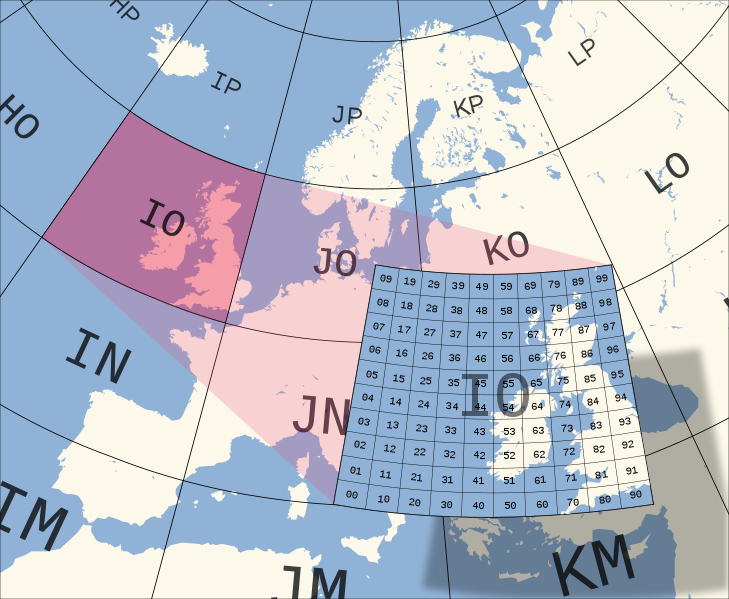
\includegraphics[width=0.6\textwidth,height=.65\textheight,keepaspectratio]{bv11/Maidenhead_grid_over_Europe.png}
      \attribcaption{Maidenhead Grid}{Oona Räisänen (Mysid)}{https://commons.wikimedia.org/wiki/File:Maidenhead_grid_over_Europe.svg}{\ccbysa}
    \end{figure}
  \end{center}

  Von \emph{IARU} entwickelter Standortkenner durch Aufteilung der Erde in Felder.

\end{frame}

\begin{frame}
  \frametitle{QTH-Locator (Maidenhead Locator)}

  \begin{center}
    \begin{figure}
      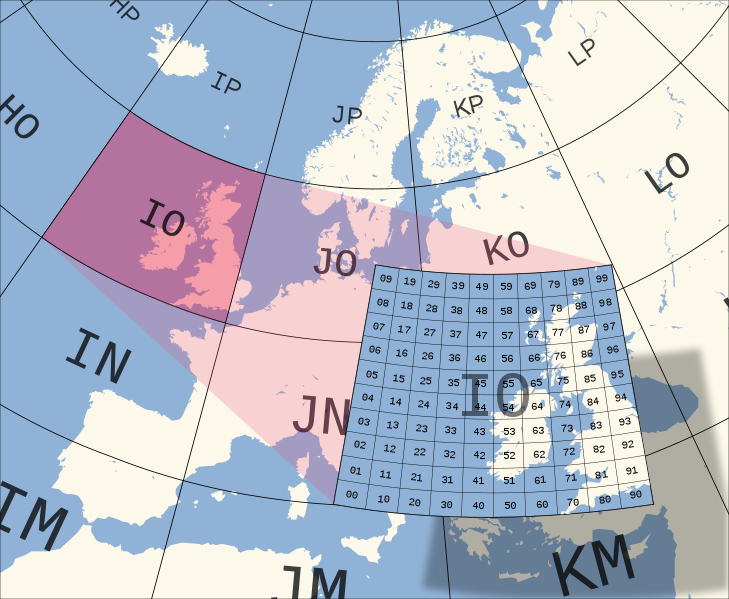
\includegraphics[width=0.5\textwidth,height=.3\textheight,keepaspectratio]{bv11/Maidenhead_grid_over_Europe.png}
      \attribcaption{Maidenhead Grid}{Oona Räisänen (Mysid)}{https://commons.wikimedia.org/wiki/File:Maidenhead_grid_over_Europe.svg}{\ccbysa}
    \end{figure}
  \end{center}

  \begin{description}
    \item[324 Fields (Größtfelder)\footnote{20 Längengrade, 10 Breitengrade}] AA (links unten) bis RR (rechts oben)
    \item[100 Squares (Großfelder) \footnote{2 Längengrade, 1 Breitengrad}] 00 (l.u.) bis 99 (r.o.)
    \item[576 Subsquares (Kleinfelder) \footnote{ca. 7x5 km in unseren Breitengraden}] AA (l.u.) bis XX (r.o.)
  \end{description}

\end{frame}

\section{Baken}

\begin{frame}
  \frametitle{Baken im VHF/UHF-Bereich}

  Angemeldete automatisch arbeitende Sender zur Bestimmung der
  Ausbreitungsbedingungen -- wie bei HF.

  \begin{itemize}
    \item im Unterschied zur HF-Bake auch Aussendung des Locators und ggf.
      zusätzliche Infos
    \item auch hier: Sendeverbot auf den QRGs
  \end{itemize}

\end{frame}

\section{Bandpläne}

\begin{frame}
  \frametitle{Bandpläne}

  Schauen wir nun mit dem erworbenen Wissen auf die Bandpläne: \\[2em]

  \url{http://www.darc.de/referate/vus/bandplaene/}

\end{frame}


\renewcommand{\refname}{Referenzen}

\begin{frame}
  \frametitle{Referenzen/Links}
  \hypertarget{refs}{}
  \footnotesize

  \begin{thebibliography}{}
    \bibitem{dj4uf} Moltrecht B/V 11: \\
      \url{https://www.darc.de/der-club/referate/ajw/lehrgang-bv/bv11/}
    \bibitem{wp}    Wikipedia DE: \\
      \url{http://de.wikipedia.org/wiki/Duplex_\%28Nachrichtentechnik\%29} \\
      \url{http://de.wikipedia.org/wiki/Echolink} \\
      \url{http://de.wikipedia.org/wiki/Troposph\%C3\%A4re} \\
      \url{http://de.wikipedia.org/wiki/Sporadic-E} \\
      \url{http://de.wikipedia.org/wiki/Transponder} \\
      \url{http://de.wikipedia.org/wiki/OSCAR} \\
      \url{http://de.wikipedia.org/wiki/Kleinsatellit} \\
      \url{http://de.wikipedia.org/wiki/QTH-Locator} \\
      \url{http://de.wikipedia.org/wiki/\%C3\%9Cberreichweite}
    \bibitem{we}    Wikipedia EN: \\
      \url{http://en.wikipedia.org/wiki/Simplex_communication} \\
      \url{http://en.wikipedia.org/wiki/Duplex_\%28telecommunications\%29}
    \bibitem{darc}  UKW-Bandpläne des DARC: \\
      \url{http://www.darc.de/referate/vus/bandplaene/}
  \end{thebibliography}

\end{frame}

% Hier könnte noch eine Kontaktfolie stehen

\end{document}

